\documentclass[
11pt, % The default document font size, options: 10pt, 11pt, 12pt
%codirector, % Uncomment to add a codirector to the title page
]{charter} 




% El títulos de la memoria, se usa en la carátula y se puede usar el cualquier lugar del documento con el comando \ttitle
\titulo{Sistema de monitoreo para planta de acopio de cereales} 

% Nombre del posgrado, se usa en la carátula y se puede usar el cualquier lugar del documento con el comando \degreename
%\posgrado{Carrera de Especialización en Sistemas Embebidos} 
\posgrado{Carrera de Especialización en Internet de las Cosas} 
%\posgrado{Carrera de Especialización en Intelegencia Artificial}
%\posgrado{Maestría en Sistemas Embebidos} 
%\posgrado{Maestría en Internet de las cosas}

% Tu nombre, se puede usar el cualquier lugar del documento con el comando \authorname
\autor{Ing. Lucas Eduardo Olmedo} 

% El nombre del director y co-director, se puede usar el cualquier lugar del documento con el comando \supname y \cosupname y \pertesupname y \pertecosupname
\director{Marcelo Castello}
\pertenenciaDirector{UTN-FRRO} 
% FIXME:NO IMPLEMENTADO EL CODIRECTOR ni su pertenencia
\codirector{John Doe} % para que aparezca en la portada se debe descomentar la opción codirector en el documentclass
\pertenenciaCoDirector{FIUBA}

% Nombre del cliente, quien va a aprobar los resultados del proyecto, se puede usar con el comando \clientename y \empclientename
\cliente{Tribunal Jurado trabajo final CEIoT}
\empresaCliente{FIUBA}

% Nombre y pertenencia de los jurados, se pueden usar el cualquier lugar del documento con el comando \jurunoname, \jurdosname y \jurtresname y \perteunoname, \pertedosname y \pertetresname.
\juradoUno{Nombre y Apellido (1)}
\pertenenciaJurUno{pertenencia (1)} 
\juradoDos{Nombre y Apellido (2)}
\pertenenciaJurDos{pertenencia (2)}
\juradoTres{Nombre y Apellido (3)}
\pertenenciaJurTres{pertenencia (3)}
 
\fechaINICIO{28 de febrero de 2023}		%Fecha de inicio de la cursada de GdP \fechaInicioName
\fechaFINALPlan{24 de abril de 2023} 	%Fecha de final de cursada de GdP
\fechaFINALTrabajo{15 de febrero de 2024}	%Fecha de defensa pública del trabajo final


\begin{document}

\maketitle
\thispagestyle{empty}
\pagebreak


\thispagestyle{empty}
{\setlength{\parskip}{0pt}
\tableofcontents{}
}
\pagebreak


\section*{Registros de cambios}
\label{sec:registro}


\begin{table}[ht]
\label{tab:registro}
\centering
\begin{tabularx}{\linewidth}{@{}|c|X|c|@{}}
\hline
\rowcolor[HTML]{C0C0C0} 
Revisión & \multicolumn{1}{c|}{\cellcolor[HTML]{C0C0C0}Detalles de los cambios realizados} & Fecha      \\ \hline
0      & Creación del documento                                 &\fechaInicioName \\ \hline
1      & Se completa hasta el punto 5 inclusive                 & 12 de marzo de 2023 \\ \hline
2      & Se completa hasta el punto 9 inclusive                 & 20 de marzo de 2023 \\ \hline
3      & Se completa hasta el punto 12 inclusive                & 27 de marzo de 2023 \\ \hline
4      & Se completa hasta el punto 15 inclusive                & 3 de abril de 2023 \\ \hline
\end{tabularx}
\end{table}

\pagebreak



\section*{Acta de constitución del proyecto}
\label{sec:acta}

\begin{flushright}
Buenos Aires, \fechaInicioName
\end{flushright}

\vspace{2cm}

Por medio de la presente se acuerda con el \authorname\hspace{1px} que su Trabajo Final de la \degreename\hspace{1px} se titulará ``\ttitle'', consistirá esencialmente en la implementación de un prototipo de un sistema para monitorear plantas de acopio de cereales, y tendrá un presupuesto preliminar estimado de 600 h de trabajo y \$3923100, con fecha de inicio \fechaInicioName\hspace{1px} y fecha de presentación pública \fechaFinalName.

Se adjunta a esta acta la planificación inicial.

\vfill

% Esta parte se construye sola con la información que hayan cargado en el preámbulo del documento y no debe modificarla
\begin{table}[ht]
\centering
\begin{tabular}{ccc}
\begin{tabular}[c]{@{}c@{}}Dr. Ing. Ariel Lutenberg \\ Director posgrado FIUBA\end{tabular} & \hspace{2cm} & \begin{tabular}[c]{@{}c@{}}\clientename \\ \empclientename \end{tabular} \vspace{2.5cm} \\ 
\multicolumn{3}{c}{\begin{tabular}[c]{@{}c@{}} \supname \\ Director del Trabajo Final\end{tabular}} \vspace{2.5cm} \\
%\begin{tabular}[c]{@{}c@{}}\jurunoname \\ Jurado del Trabajo Final\end{tabular}     &  & \begin{tabular}[c]{@{}c@{}}\jurdosname\\ Jurado del Trabajo Final\end{tabular}  \vspace{2.5cm}  \\
%\multicolumn{3}{c}{\begin{tabular}[c]{@{}c@{}} \jurtresname\\ Jurado del Trabajo Final\end{tabular}} \vspace{.5cm}                                                                     
\end{tabular}
\end{table}




\section{1. Descripción técnica-conceptual del proyecto a realizar}
\label{sec:descripcion}

El presente proyecto es un emprendimiento personal dirigido a solucionar un problema detectado en algunas plantas de acopio de cereales. Una empresa  o cooperativa dedicada al almacenamiento de granos tiene uno o más depósitos distribuidos y para controlar el estado de almacenamiento de sus productos necesita enviar operarios a las diferentes plantas. Dada esta situación, se plantea implementar un sistema de monitoreo IoT para optimizar tiempos y costos. 

Una planta de acopio se encarga de recepcionar diferentes diferentes tipos de granos, analizarlos, secarlos y almacenarlos. Para ello, dispone de silos equipados con sistemas de ventilación y control de termométricos, con el objetivo de minimizar las pérdidas de granos tanto en forma cuantitativa como cualitativa durante la etapa de almacenamiento. 

Una empresa que brinde servicio de almacenamiento puede tener varias plantas de acopio distribuidas en diferentes ciudades o zonas rurales. El objetivo del sistema IoT a desarrollar es simplificar la tarea de administración que puede tener una empresa o cooperativa. Se propone instalar nodos y sensores identificando cada silo, monitorizar el estado del cereal almacenado y centralizar esta información en la nube. Con este sistema será posible trazar el estado de almacenamiento del cereal, disminuir las tareas manuales del personal en cada planta y administrar más de una planta desde una sola oficina. 

Si bien en el mercado se encuentran algunas ofertas de sistemas IoT para silos, se plantea diseñar una solución a medida mediante la reutilización de instalaciones existentes y brindando así la posibilidad de reciclar sensores. La propuesta es instalar un nodo por cada silo, este debe obtener datos de sensores para luego transmitirlos hacia la nube. 

La solución propuesta se compone de las siguientes partes: 
\begin{itemize}
	\item Obtención de datos desde sensores. 
	\item Adaptar y transmitir datos a la nube.
	\item Procesamiento y persistencia de datos.
	\item Presentación de datos y alarmas. 
\end{itemize}

En la Figura \ref{fig:diagBloques} se presenta el diagrama en bloques del sistema. Se observa que cada planta de acopio esta compuesta de silos, cada uno de estos posee un nodo con uno o mas sensores. Los nodos transmiten los datos a la nube, los cuales serán almacenados en un servidor de bases de datos y presentados en un \textit{dashboard} o aplicación en las oficinas de la empresa o cooperativa.

\begin{figure}[htpb]
\centering 
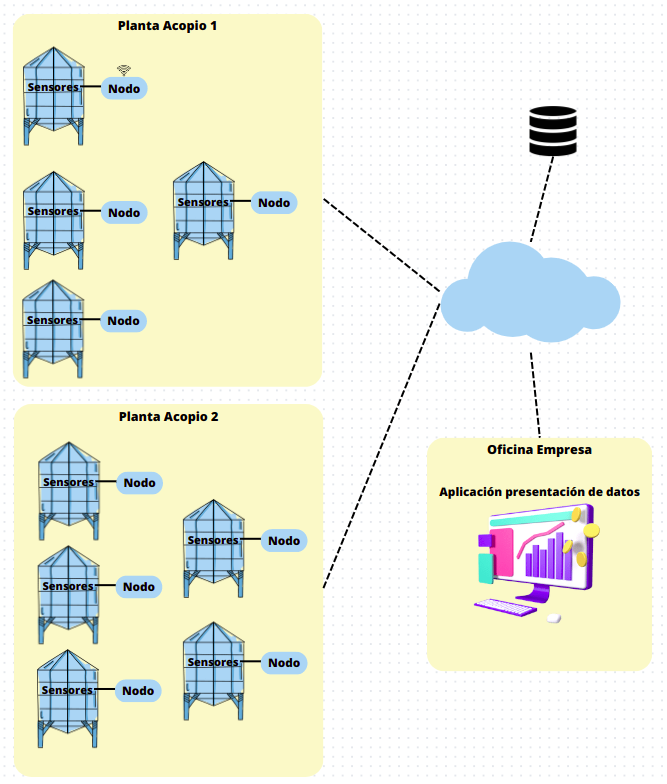
\includegraphics[width=.9\textwidth]{./Figuras/PlantaAcopio.png}
\caption{Diagrama en bloques del sistema}
\label{fig:diagBloques}
\end{figure}

\vspace{25px}

\section{2. Identificación y análisis de los interesados}
\label{sec:interesados}

\begin{table}[ht]
%\caption{Identificación de los interesados}
%\label{tab:interesados}
\begin{tabularx}{\linewidth}{@{}|l|X|X|l|@{}}
\hline
\rowcolor[HTML]{C0C0C0} 
Rol           & Nombre y Apellido    & Organización 	& Puesto 	\\ \hline
%Auspiciante   &                     &              	&        	\\ \hline
Cliente       & \clientename         &\empclientename	&--       	\\ \hline
%Impulsor      &                     &              	&        	\\ \hline
Responsable   & \authorname          & FIUBA        	& Alumno 	\\ \hline
%Colaboradores &                     &              	&        	\\ \hline
Orientador    & \supname	         & \pertesupname 	& Director Trabajo final \\ \hline
%Equipo        & miembro1 \newline 
%				miembro2             &              	&        	\\ \hline
%Opositores    &--                   &Empresas de la competencia   	&--        	\\ \hline
Usuario final &Empleados Oficina     & Empresa de Acopio   	& Operador / Administrador        	\\ \hline
\end{tabularx}
\end{table}

\begin{itemize}
	\item Cliente: es el jurado del trabajo final de la especialización de IoT. Todavía a definir. 
\end{itemize}



\section{3. Propósito del proyecto}
\label{sec:proposito}

El propósito de este proyecto es implementar un sistema de monitoreo para el almacenamiento de cereales, con el objetivo de conservar en condiciones óptimas los granos almacenados. El sistema deberá diseñarse e implementarse utilizando los conocimientos adquiridos durante el cursado de la CEIoT y con miras a su implementación en campo a futuro. 

\section{4. Alcance del proyecto}
\label{sec:alcance}

El alcance del proyecto incluye:

\begin{itemize}
 \item Un prototipo funcional. 
 \item Al menos un nodo instalado en un silo que simule datos obtenidos y transmita los mismos a la nube. 
 \item Selección del protocolo para transmisión de datos. 
 \item Desarrollo de \textit{backend} del sistema que procese y almacene los datos recibidos.
 \item Presentación de datos en una aplicación.
\end{itemize}

El presente proyecto no incluye: 

\begin{itemize}
 \item La puesta en marcha del producto en las instalaciones de una planta de almacenamiento.
 \item La lectura de datos en sensores reales desde los nodos.
\end{itemize}




\section{5. Supuestos del proyecto}
\label{sec:supuestos}

Para el desarrollo del presente proyecto se supone que: 

\begin{itemize}
	\item Se implementa un prototipo para el trabajo final de CEIoT, pero el proyecto se continuara. 
	\item Las plantas de acopio disponen de una conexión a internet. 
	\item Se dispone de la colaboración de personas idóneas en el almacenamiento de cereales.
	\item Se dispone continuidad de los recursos humanos necesarios durante el desarrollo del proyecto. 
	\item Se contará con los recursos económicos necesarios para la realización del proyecto. 
	\item Se cuenta con el \textit{hardware} necesario para implementar al menos un prototipo.
	\item El cliente acepta que las mediciones de temperatura y cantidad de cereal en un silo sean simuladas. 
\end{itemize}


\section{6. Requerimientos}
\label{sec:requerimientos}

\begin{enumerate}
	\item Requerimientos funcionales
		\begin{enumerate}
			\item El sistema deberá monitorizar silos de diferentes plantas de acopio.
			\item El sistema deberá obtener la temperatura de los silos y transmitirla cada 10 minutos.
			\item El sistema deberá obtener la cantidad en kg de cereal almacenado en un silo y transmitirlo cada 15 minutos.
			\item El sistema deberá mostrar la capacidad máxima de almacenamiento de cada silo y el tipo de cereal almacenado.
			\item El sistema deberá transmitir los datos de forma segura desde los nodos sensores a un servidor. 
			\item El sistema deberá contar con una interfaz gráfica donde se presenten los datos obtenidos.
			\item La interfaz gráfica se debe poder acceder por los usuarios de la empresa en diferentes computadoras.
			\item El sistema deberá generar alertas a los usuarios cuando un silo supere una determinada temperatura. 
			\item El sistema deberá almacenar el historial de mediciones por cada silo en una base de datos. 
			\item El sistema deberá mostrar en tiempo real las mediciones de un silo. 
			\item El sistema deberá mostrar el historial de mediciones de un silo.
			\item El sistema deberá mostrar todos los silos de una planta indicando si las mediciones de temperatura de un silo están fuera de un rango establecido. 
		\end{enumerate}
	\item Requerimientos no funcionales
		\begin{enumerate}
			\item El sistema deberá ser escalable, permitiendo agregar mas plantas de acopio dentro de una empresa, mas silos en una planta y mas sensores en un silo.  
			\item El sistema debe estar protegido contra el acceso no autorizado.
			\item El sistema debe tener una interfaz intuitiva y documentación clara para facilitar su uso por parte del usuario.
		\end{enumerate}	
	\item Requerimientos de documentación
		\begin{enumerate}
			\item Se debe generar un documento de planificación del proyecto.
			\item Se debe generar un manual de uso.
			\item Se debe generar un manual de instalación.
			\item Se debe generar una memoria técnica con la documentación de ingeniería detallada.			
		\end{enumerate}
\end{enumerate}

\section{7. Historias de usuarios (\textit{Product backlog})}
\label{sec:backlog}

\textit{Story points}: Se utilizarán 1, 2, 3, 5, 8 y 13 para la estimación de las historias de usuario, según la
serie de Fibonacci.
Los \textit{story points} se asignan a una tarea o historia de usuario en función de la complejidad que representa para el equipo de proyecto. La asignación de \textit{story points} se basa en una evaluación en equipo de varios factores como: esfuerzo requerido, dificultad, complejidad e incertidumbre.

\begin{itemize}
\item Como cliente quiero visualizar todas las plantas de acopio de la empresa en una sola aplicación para tener el control desde una o varias oficinas. (\textit{Story points}: 3.  Esta tarea solo implica hacer una pantalla de visualización y una consulta a la base.)

\item Como cliente quiero ver la temperatura de un silo en tiempo real en una aplicación para controlar el estado de conservación del cereal a distancia. (\textit{Story points}: 5. En esta historia se considera que debe implementarse tanto la UI como la simulacion y transmision de la temperatura.)

\item Como cliente quiero saber la cantidad de cereal almacenado en un silo para poder decidir si es posible almacenar mas cereal en este.  (\textit{Story points}: 5. En esta historia es necesario investigar para poder implementar lo solicitado. )

\item Como cliente quiero tener información de la capacidad restante de almacenamiento de un silo y el tipo de cereal para poder realizar logística sin necesidad de ir a la planta. (\textit{Story points}: 2. Al tener implementada la historia anterior, esta es simple.)

\item Como cliente quiero visualizar una alarma cuando un silo supere una temperatura determinada, indicando la planta y silo correspondiente para poder tomar acciones preventivas y mantener el cereal en optimo estado. (\textit{Story points}: 2. Esta historia solo es de UI)

\item Como cliente quiero poder visualizar el historial de mediciones de un silo para controlar el estado del almacenamiento del cereal. (\textit{Story points}: 8. Es necesario implementar una base de datos y la UI para visualizar los datos)

\item Como cliente quiero poder acceder a la aplicación desde distintas computadoras para poder monitorizar las plantas de acopio desde diferentes oficinas. (\textit{Story points}: 3. No se observa gran dificultad.)

\item Como gerente de la empresa quiero que el sistema pida usuario y contraseña al ingresar para que solo puedan acceder personas autorizadas. (\textit{Story points}: 13. Esta historia es considerada mas compleja ya que el equipo no cuenta con experiencia en tareas relacionadas.)
\end{itemize}

\section{8. Entregables principales del proyecto}
\label{sec:entregables}

\begin{itemize}
	\item Manual de uso.
	\item Manual de instalación.
	\item Prototipo funcional.
	\item Diagrama esquemático de la solución.
	\item Informe final.
	\item Presentación.
\end{itemize}

\section{9. Desglose del trabajo en tareas}
\label{sec:wbs}

\begin{enumerate}
\item Planificación y definición del proyecto (55 h)
	\begin{enumerate}
	\item Investigación preliminar (25 h)
	\item Relevar requerimientos(15 h)
	\item Documentar planificación del proyecto (15 h)
	\end{enumerate}
\item Protocolo de comunicación (24 h)
	\begin{enumerate}
	\item Investigación y elección de protocolo de comunicación (24 h)
	\end{enumerate}
\item Análisis y Diseño del modelo de datos (44 h)
	\begin{enumerate}
	\item Elección de tecnología (4 h)
	\item Diseño del modelo de datos (20 h)
	\item Implementación base de datos y carga inicial de datos (20 h)
	\end{enumerate}
\item Diseño e implementación del nodo y mediciones simuladas (76 h)
	\begin{enumerate}
	\item Elección del \textit{hardware} (4 h)
	\item Simulación adquisición de temperatura (20 h)
	\item Simulación nivel de llenado silo en kg (16 h)
	\item Transmisión de datos simulados (20 h)
	\item Pruebas de funcionalidad del nodo (16 h)
	\end{enumerate}	
\item Planificación y desarrollo del \textit{backend} (64 h)
	\begin{enumerate}
	\item Especificación de los requerimientos del \textit{backend} (8 h)
	\item Desarrollo del \textit{backend} (40 h)
	\item Pruebas de funcionalidad del \textit{backend} (16 h)
	\end{enumerate}
\item Planificación y desarrollo del \textit{frontend} (80 h)
	\begin{enumerate}
	\item Especificación de los requerimientos del \textit{frontend} (8 h)
	\item Desarrollo del \textit{frontend} (40 h)
	\item Desarrollo de la comunicación con la base de datos (16 h)
	\item Pruebas de funcionalidad del \textit{frontend} (16 h) 
	\end{enumerate}
\item Diseño e implementación de un sistema de acceso al software (68 h)
	\begin{enumerate}
	\item Especificación de requerimientos de acceso (12 h)
	\item Desarrollo del sistema de acceso (32 h)
	\item Pruebas del sistema de acceso (24 h) 
	\end{enumerate}		
\item Pruebas finales (63 h)
	\begin{enumerate}
	\item Planificación de las pruebas (12 h) 
	\item Generación del ambiente de pruebas (35 h)
	\item Ejecución de las pruebas (16 h)
	\end{enumerate}
\item Documentación (60 h)
	\begin{enumerate}
	\item Generación del manual de instalación (28 h)
	\item Generación del manual del usuario (32 h)
	\end{enumerate}
\item Actividades de cierre (80 h)
	\begin{enumerate}
	\item Generación de la memoria final (48 h)
	\item Generación de video de uso (16 h)
	\item Elaboración de la presentación (16 h) 
	\end{enumerate}
\end{enumerate}

Cantidad total de horas: (614 h).

\section{10. Diagrama de Activity On Node}
\label{sec:AoN}

La unidad de tiempo del diagrama AoN que se muestra en la Figura \ref{fig:AoN} esta expresada en horas.

\begin{figure}[htpb]
\centering 
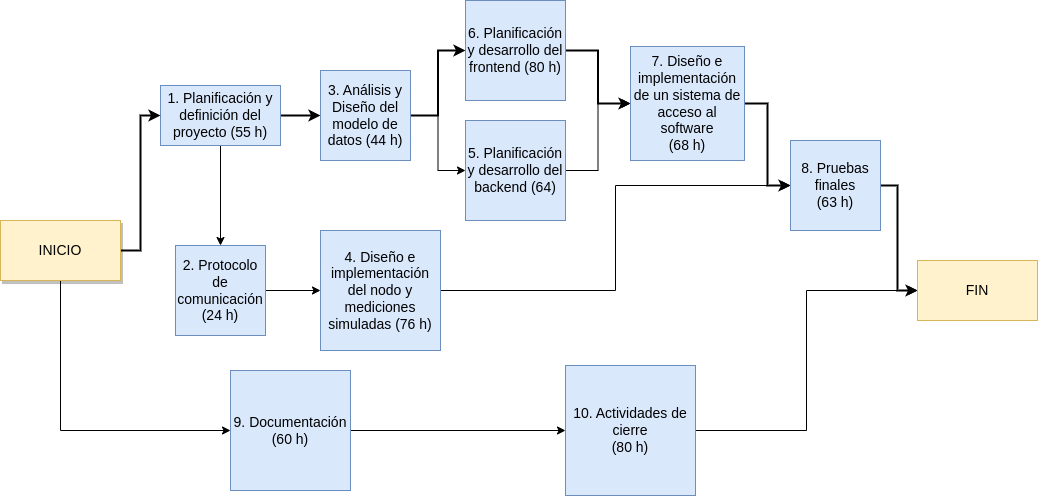
\includegraphics[width=1\textwidth]{./Figuras/DiagramaActivityONNode.png}
\caption{Diagrama de \textit{Activity on Node}.}
\label{fig:AoN}
\end{figure}

\begin{itemize}
	\item El camino critico es de 310 h y esta compuesto por la secuencia de tareas 1-3-6-7-8.
	\item El camino semi critico es de 294 h y esta compuesto por la secuencia de tareas 1-3-5-7-8.
\end{itemize}

\section{11. Diagrama de Gantt}
\label{sec:gantt}



En la figura \ref{fig:TareasGant}, se muestra el desglose de tareas del diagrama de gant.

En las figuras \ref{fig:diagGantt1} y \ref{fig:diagGantt2} se observa el diagrama de gantt. Se considero un recurso trabajando los días martes y jueves 4h por día y los sábados 8h. 

\begin{landscape}
\begin{figure}[htpb]
\centering 
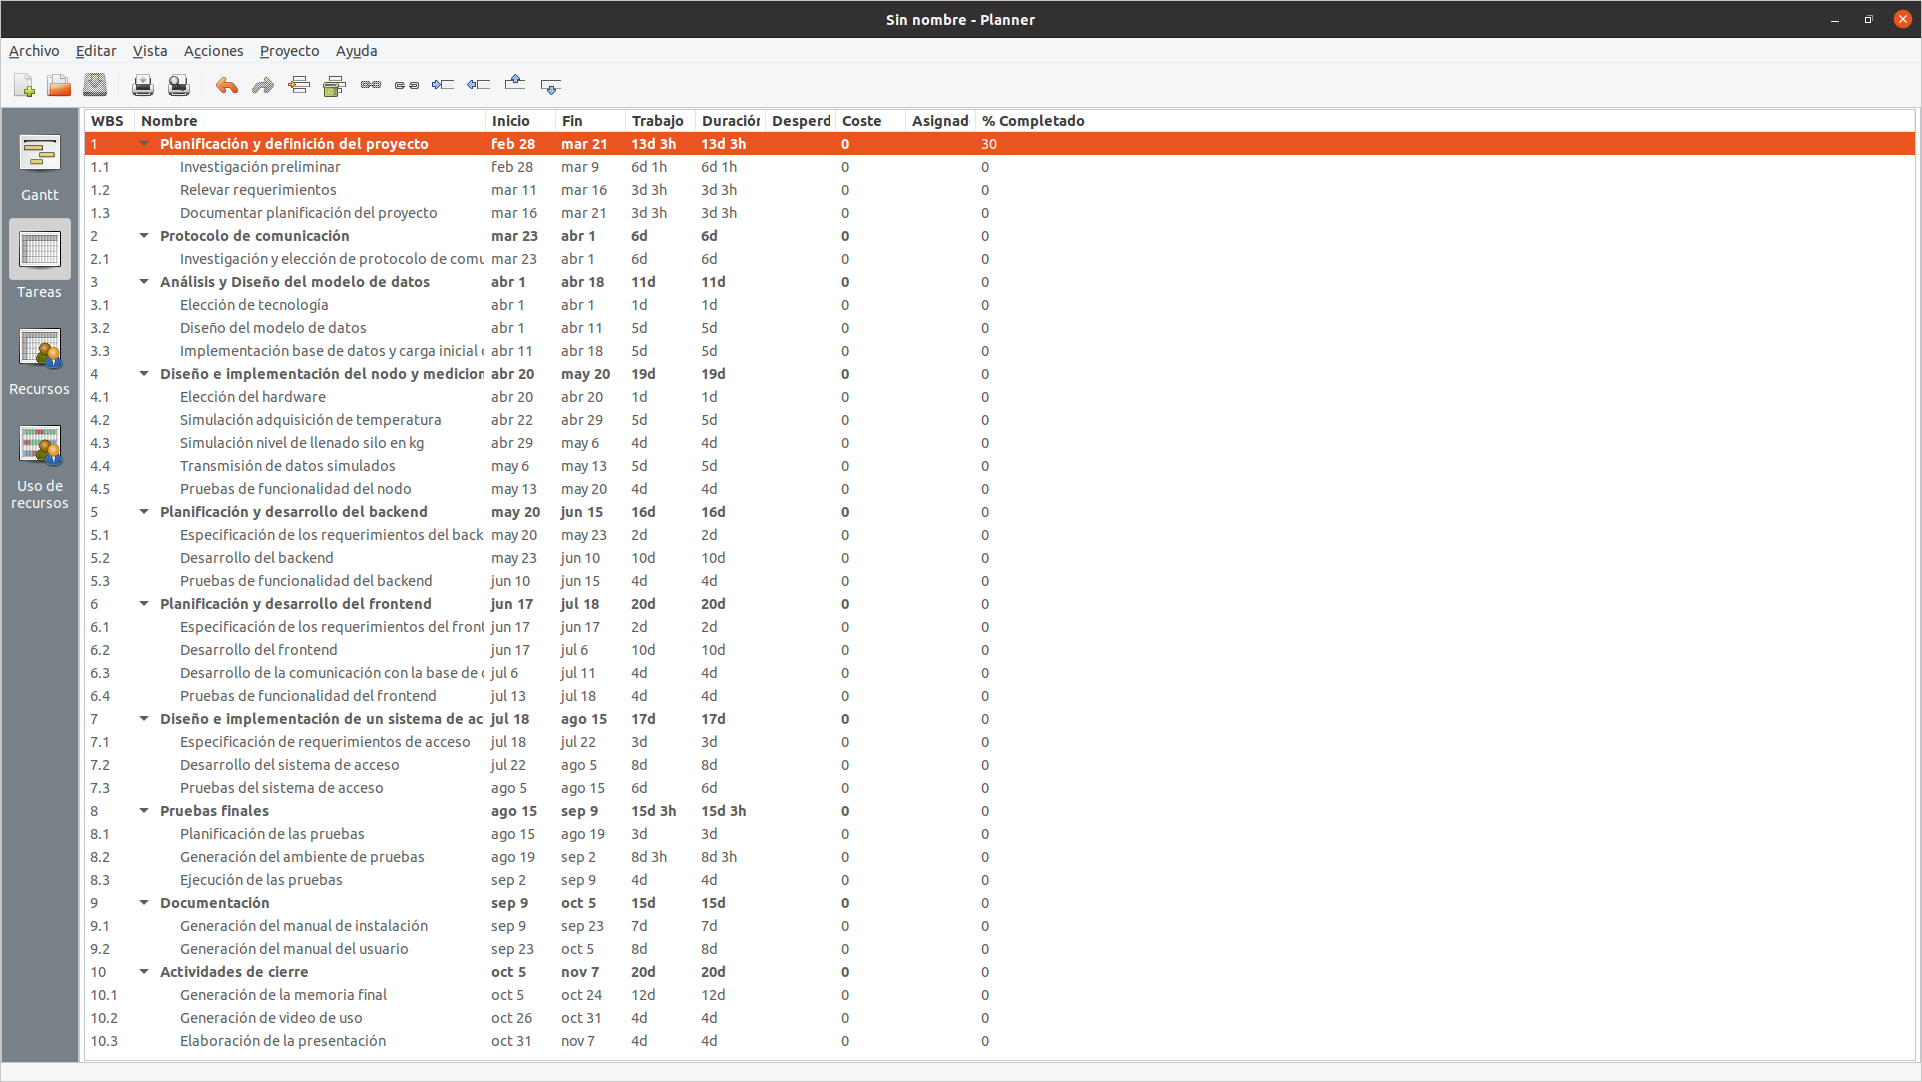
\includegraphics[height=.85\textheight]{./Figuras/TareasGant.png}
\caption{Tareas Diagrama de Gantt}
\label{fig:TareasGant}
\end{figure}
\end{landscape}

\begin{landscape}
\begin{figure}[htpb]
\centering 
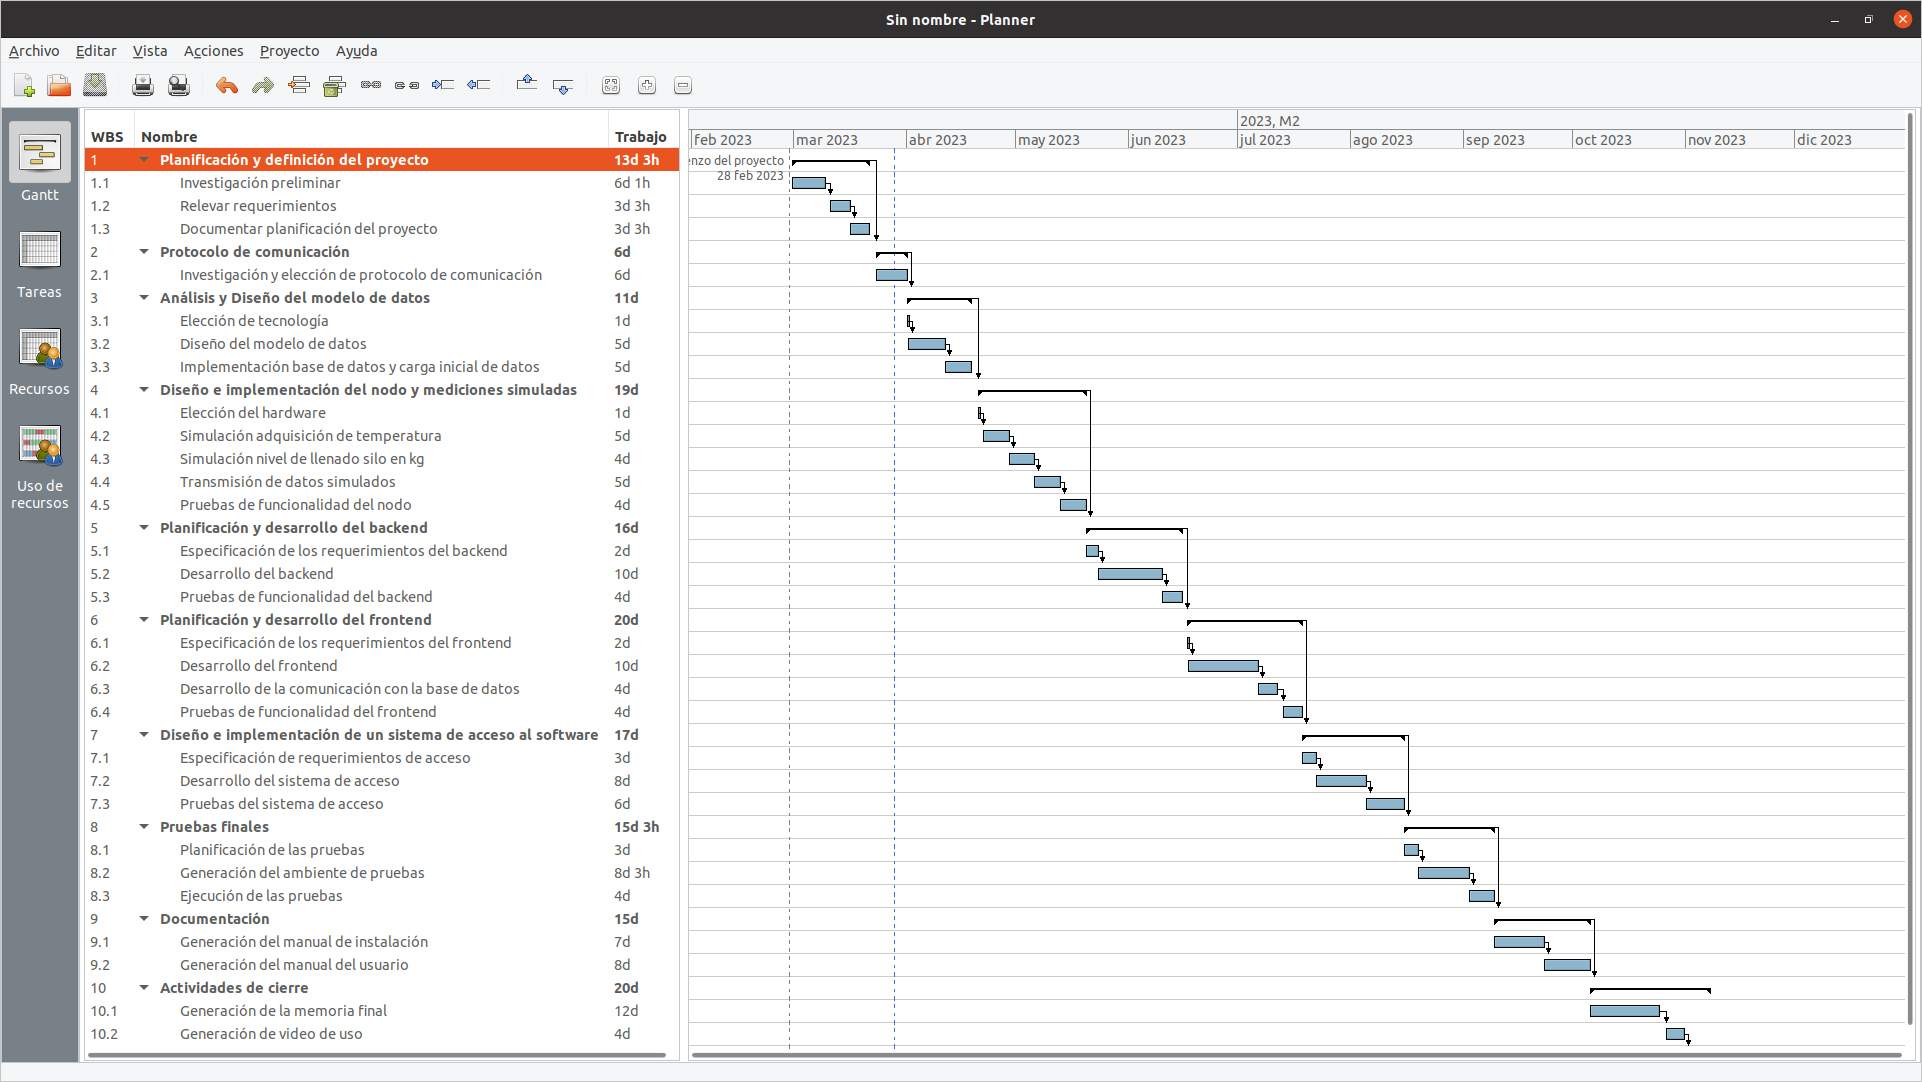
\includegraphics[height=.85\textheight]{./Figuras/DiagramaGant1.png}
\caption{Diagrama de Gantt parte 1}
\label{fig:diagGantt1}
\end{figure}

\end{landscape}

\begin{landscape}
\begin{figure}[htpb]
\centering 
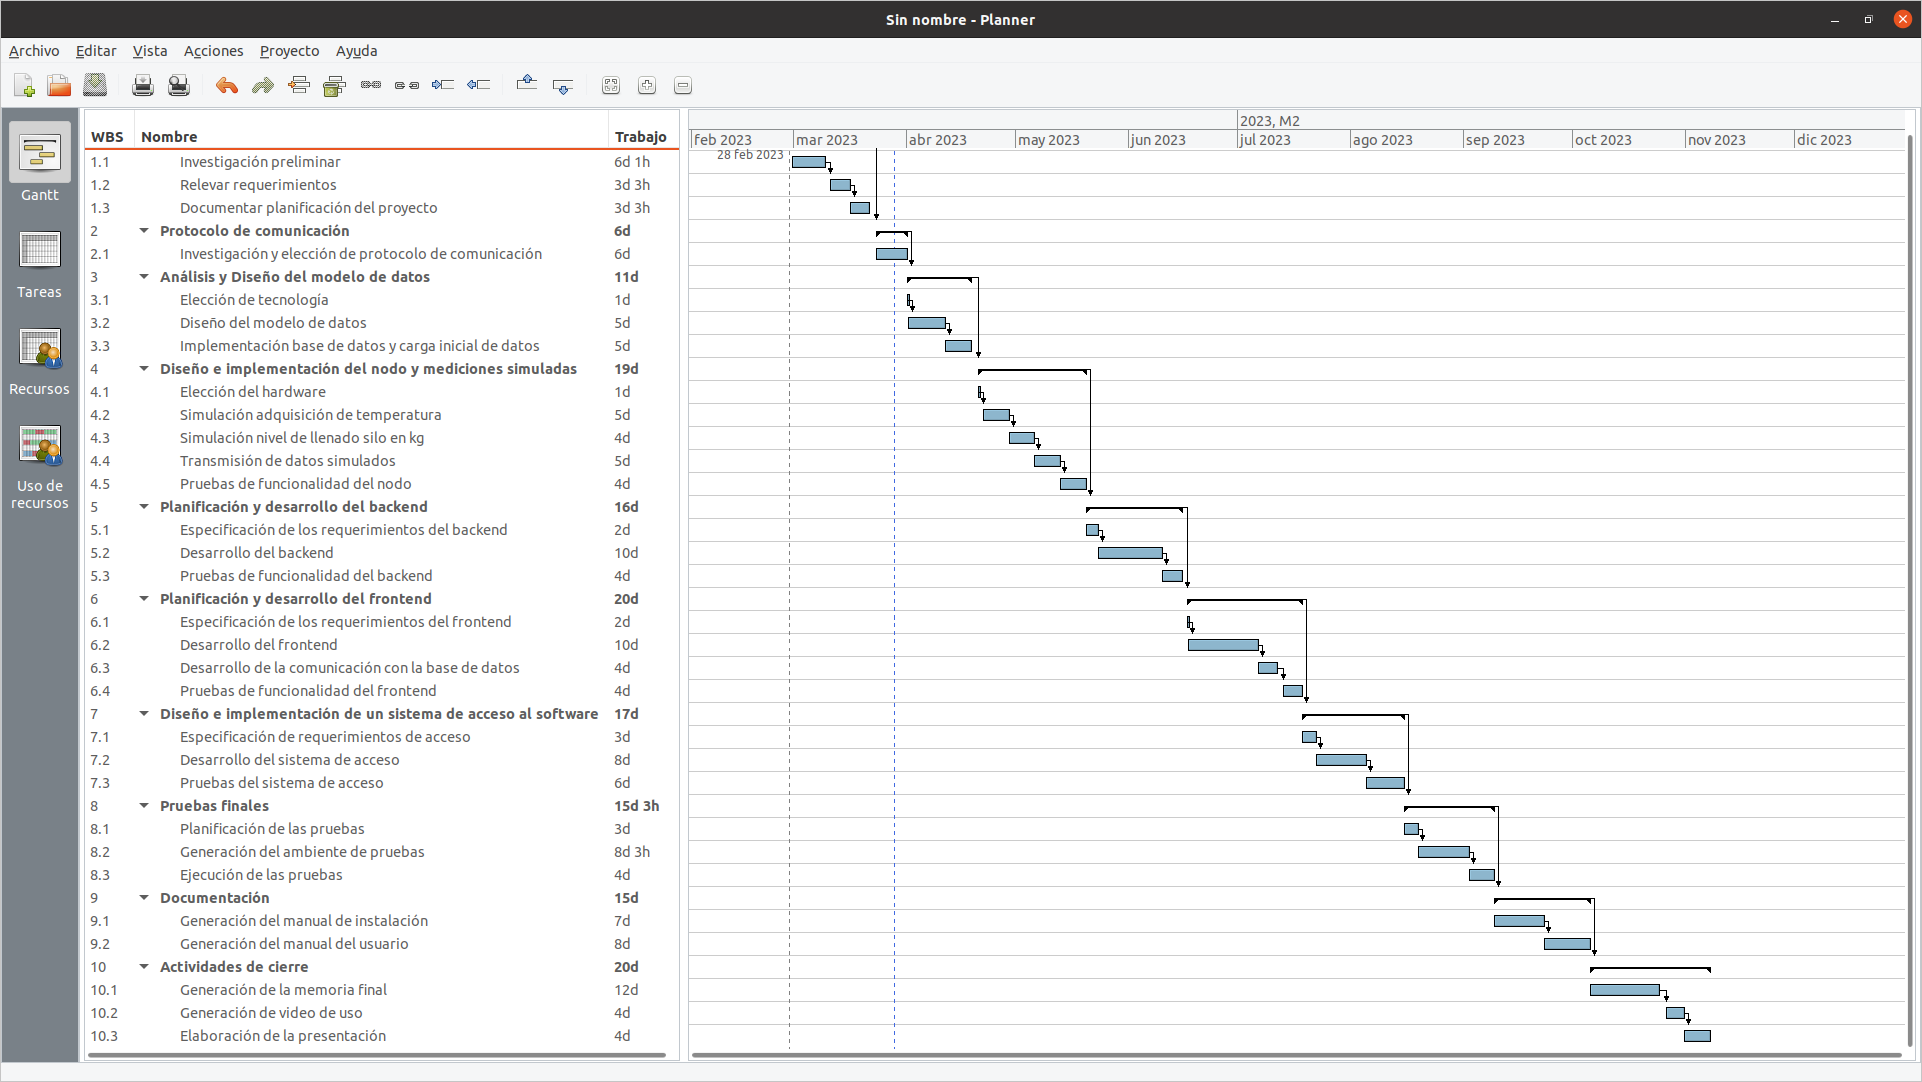
\includegraphics[height=.85\textheight]{./Figuras/DiagramaGant2.png}
\caption{Diagrama de Gantt parte 2}
\label{fig:diagGantt2}
\end{figure}

\end{landscape}


\section{12. Presupuesto detallado del proyecto}
\label{sec:presupuesto}

\begin{table}[htpb]
\centering
\begin{tabularx}{\linewidth}{@{}|X|c|r|r|@{}}
\hline
\rowcolor[HTML]{C0C0C0} 
\multicolumn{4}{|c|}{\cellcolor[HTML]{C0C0C0}COSTOS DIRECTOS} \\ \hline
\rowcolor[HTML]{C0C0C0} 
Descripción &
  \multicolumn{1}{c|}{\cellcolor[HTML]{C0C0C0}Cantidad} &
  \multicolumn{1}{c|}{\cellcolor[HTML]{C0C0C0}Valor unitario} &
  \multicolumn{1}{c|}{\cellcolor[HTML]{C0C0C0}Valor total} \\ \hline
Hardware nodos&
  \multicolumn{1}{c|}{-} &
  \multicolumn{1}{c|}{150000} &
  \multicolumn{1}{c|}{150000} \\ \hline
Horas ingeniería&
  \multicolumn{1}{c|}{614} &
  \multicolumn{1}{c|}{4000} &
  \multicolumn{1}{c|}{2456000} \\ \hline
Servicios cloud&
  \multicolumn{1}{c|}{-} &
  \multicolumn{1}{c|}{200000} &
  \multicolumn{1}{c|}{200000} \\ \hline
  Montaje y pruebas en campo&
  \multicolumn{1}{c|}{-} &
  \multicolumn{1}{c|}{100000} &
  \multicolumn{1}{c|}{100000} \\ \hline
\multicolumn{3}{|c|}{SUBTOTAL} &
  \multicolumn{1}{c|}{2906000} \\ \hline
\rowcolor[HTML]{C0C0C0} 
\multicolumn{4}{|c|}{\cellcolor[HTML]{C0C0C0}COSTOS INDIRECTOS} \\ \hline
%\rowcolor[HTML]{C0C0C0} 
%Descripción &
%  \multicolumn{1}{c|}{\cellcolor[HTML]{C0C0C0}Cantidad} &
%  \multicolumn{1}{c|}{\cellcolor[HTML]{C0C0C0}Valor unitario} &
%  \multicolumn{1}{c|}{\cellcolor[HTML]{C0C0C0}Valor total} \\ \hline
\multicolumn{3}{|c|}{35\% de los costos directos} &
 %  -&
  \multicolumn{1}{c|}{1017100} \\ \hline
\multicolumn{3}{|c|}{SUBTOTAL} &
  \multicolumn{1}{c|}{1017100} \\ \hline
\rowcolor[HTML]{C0C0C0}
\multicolumn{3}{|c|}{TOTAL} &
  \multicolumn{1}{c|}{3923100}
   \\ \hline
\end{tabularx}%
\end{table}

Consideraciones:
\begin{itemize}
	\item Los costos son estimados ya que en esta instancia del proyecto no esta definido el \textit{hardware} a utilizar 
	\item Los valores están indicados en pesos argentinos, la tasa de cambio actual es de 1 dólar = 213.50 pesos (Banco nación, 27 de marzo de 2023) 
	\item El costo de la hora de ingeniería se obtiene del costo promedio de la hora para un ingeniero de software con varios años de experiencia. 
\end{itemize}


\section{13. Gestión de riesgos}
\label{sec:riesgos}

a) Identificación de los riesgos y estimación de sus consecuencias:
 
Riesgo 1: riesgo de que los datos puedan ser robados o alterados por personas no autorizadas.
\begin{itemize}
	\item Severidad (S): 8. Si los datos del proyecto son robados o alterados por personas no autorizadas, el impacto puede ser significativo para la empresa y los usuarios finales.
	\item Probabilidad de ocurrencia (O): 5. Si se implementan medidas de seguridad adecuadas, la ocurrencia de este riesgo puede reducirse. 
\end{itemize}   

Riesgo 2: De no cumplir con los tiempos estipulados para la entrega. 
\begin{itemize}
	\item Severidad (S): 6. Si no se cumple con el tiempo de entrega puede retrasar la entrega al cliente y peligrar la finalización de la especialización. 
	\item Ocurrencia (O): 3. Se dispone del tiempo estimado y un tiempo extra para llegar a los objetivos en caso de algún retraso o inconveniente. 
\end{itemize}

Riesgo 3: De perder los datos almacenados en la base de datos.
\begin{itemize}
	\item Severidad (S): 7. Puede producir la perdida de datos de clientes y perdida de confianza en el producto.
	\item Ocurrencia (O): 3. Implementando los conocimientos de diseño adquiridos en la especialización se reducen las probabilidades de ocurrencia. 
\end{itemize}

Riesgo 4: Los usuarios finales no aceptan el sistema o lo rechazan. 
\begin{itemize}
	\item Severidad (S): 9. Si los usuarios finales no aceptan el sistema o no se involucran en su uso, el proyecto puede fallar en su objetivo.
	\item Ocurrencia (O): 5. La ocurrencia de este riesgo depende de la aceptación y compromiso de los usuarios finales.
\end{itemize}

Riesgo 5: fallas en la conexión entre el nodo sensor y la aplicación
\begin{itemize}
	\item Severidad (S): 8. mal funcionamiento del sistema entregando datos incorrectos o con faltantes de datos. 
	\item Ocurrencia (O): 3. El sistema se diseña implementando conocimientos de arquitectura obtenidos durante el cursado de la especialidad. Se consulta con pesronas capacitadas. 
\end{itemize}

b) Tabla de gestión de riesgos:      (El RPN se calcula como RPN=SxO)

\begin{table}[htpb]
\centering
\begin{tabularx}{\linewidth}{@{}|X|c|c|c|c|c|c|@{}}
\hline
\rowcolor[HTML]{C0C0C0} 
Riesgo & S & O & RPN & S* & O* & RPN* \\ \hline
1      & 8 & 5 & 40  & 8  & 2  & 16   \\ \hline
2      & 6 & 3 & 18  &    &    &      \\ \hline
3      & 7 & 3 & 21  &    &    &      \\ \hline
4      & 9 & 5 & 45  & 9  & 3  & 27   \\ \hline
5      & 8 & 3 & 24  &    &    &      \\ \hline
\end{tabularx}%
\end{table}

Criterio adoptado: 
Se tomarán medidas de mitigación en los riesgos cuyos números de RPN sean mayores a 35

Nota: los valores marcados con (*) en la tabla corresponden luego de haber aplicado la mitigación.

c) Plan de mitigación de los riesgos que originalmente excedían el RPN máximo establecido:
 
Riesgo 1: Implementar métodos de ciberseguridad aprendidos en la especialidad con el asesoramiento de expertos. 
  - Severidad (S): 8. Si los datos del proyecto son robados o alterados por personas no autorizadas, el impacto puede ser significativo para la empresa y los usuarios finales.
  - Probabilidad de ocurrencia (O): 2. Se reduce la probabilidad de ocurrencia implementando un diseño que tiene en cuenta la ciberseguridad. 

Riesgo 4: Involucrar a los usuarios finales desde el inicio del proyecto y considerar sus necesidades y comentarios en el diseño y desarrollo del sistema.
  Nueva asignación de S y O, con su respectiva justificación:
  - Severidad (S): 9. Si los usuarios finales no aceptan el sistema o no se involucran en su uso, el proyecto puede fallar en su objetivo.
  - Probabilidad de ocurrencia (O): 3. Se reduce la probabilidad de ocurrencia al involucrar desde el principio del proyecto a los usuarios finales. 


\section{14. Gestión de la calidad}
\label{sec:calidad}

\begin{itemize} 
\item Req \#1: El sistema deberá monitorizar silos de diferentes plantas de acopio.
\begin{itemize}
	\item Verificación: Verificar el diseño del sistema, asegurando que soporte el monitoreo y visualización de mas de una planta de acopio con sus correspondientes silos. 
	\item Validación: Una vez finalizada la interfaz de usuario verificar que el sistema muestre las plantas de acopio con los silos que están siendo monitorizados. 
\end{itemize}

\item Req \#2: El sistema deberá obtener la temperatura de los silos y transmitirla cada 10 minutos.
\begin{itemize}
	\item Verificación: Análisis del código de la aplicación
	\item Validación: se comprobara que un nodo sensor envié un dato de temperatura cada 10 minutos y este valor sea visualizado en la interfaz grafica. 
\end{itemize}

\item Req \#3: El sistema debera obtener la cantidad en kg de cereal almacenado en un silo y
transmitirlo cada 15 minutos.
\begin{itemize}
	\item Verificación: Análisis del código de la aplicación
	\item Validación:se comprobara que un nodo sensor envié un dato de cantidad de cereal 15 minutos y este valor sea visualizado en la interfaz grafica. 
\end{itemize}

\item Req \#4: La interfaz grafica se debe poder acceder por los usuarios de la empresa en diferentes
computadoras.
\begin{itemize}
	\item Verificación: realizar pruebas de acceso a la interfaz gráfica desde diferentes dispositivos y navegadores web para asegurarse de que se cumple el requerimiento.
	\item Validación: realizar una revisión conjunta con los usuarios para asegurarse de que la interfaz gráfica sea intuitiva, fácil de usar y cumpla con sus expectativas.
\end{itemize}

\item Req \#5: El sistema deberá transmitir los datos de forma segura desde los nodos sensores a un
servidor.
\begin{itemize}
	\item Verificación: realizar pruebas de comunicación utilizando herramientas de monitoreo de red para asegurarse de que los datos se estén transmitiendo de manera segura.
	\item Validación: se pueden realizar pruebas de penetración y auditorías de seguridad para evaluar la robustez del sistema de transmisión de datos.
\end{itemize}

\item Req \#6: El sistema deberá generar alertas a los usuarios cuando un silo supere una determinada temperatura.
\begin{itemize}
	\item Verificación: se pueden realizar pruebas de simulación de diferentes temperaturas y verificar que el sistema esté enviando y mostrando las alertas correspondientes. 
	\item Validación: se pueden realizar pruebas de campo en la instalación del sistema y simular situaciones reales en las que un silo supere una determinada temperatura para asegurarse de que el sistema esté generando alertas de manera efectiva.
\end{itemize}

\item Req \#7: El sistema deberá almacenar el historial de mediciones por cada silo en una base de
datos.
\begin{itemize}
	\item Verificación: Verificar la estructura de base de datos confirmando que puede almacenar los datos de los silos.
	\item Validación: Validar que la información almacenada en la base de datos es precisa y actualizada. Validar que el sistema puede acceder a los datos almacenados. 
\end{itemize}

\item Req \#8: El sistema deberá mostrar el historial de mediciones de un silo.
\begin{itemize}
	\item Verificación: Verificar que la base de datos permite almacenar y acceder al histórico de mediciones de un silo.- 
	\item Validación: Comprobar con el usuario que la interfaces grafica permite mostrar datos almacenados de un silo y que los datos son correctos. 
\end{itemize}

\item Req \#9: El sistema deberá mostrar todos los silos de una planta indicando si las mediciones
de temperatura de un silo están fuera de un rango establecido.
\begin{itemize}
	\item Verificación: verificar que el sistema permite obtener los datos solicitados para mostrar. 
	\item Validación: Validar con el usuario la interfaz grafica comprobando que cubre las necesidades del cliente. 
\end{itemize}

\item Req \#10: El sistema debe estar protegido contra el acceso no autorizado.
\begin{itemize}
	\item Verificación: revisar el diseño del sistema y la implementación de medidas de seguridad para garantizar que solo los usuarios autorizados puedan acceder al sistema
	\item Validación: revisión de las políticas de seguridad de la empresa. Prueba de penetración en el sistema para validar que se han implementado medidas de seguridad efectivas para proteger el sistema contra el acceso no autorizado
\end{itemize}

\end{itemize}



\section{15. Procesos de cierre}    
\label{sec:cierre}


\begin{itemize}
	\item Pautas de trabajo que se seguirán para analizar si se respetó el Plan de Proyecto original:\\
	 - Se realizará un análisis del grado de cumplimiento de objetivos y requerimientos.\\
	 - Se verificara si se ha cumplido con los cronogramas, uso de recursos y presupuesto
originalmente planteados.\\
	Encargado: Lucas Olmedo
	\item Identificación de las técnicas y procedimientos útiles e inútiles que se emplearon, y los problemas que surgieron y cómo se solucionaron:\\
	 - Se incluirá en la memoria un detalle de los problemas encontrados y las soluciones implementadas.\\
	Encargado: Lucas Olmedo
	\item Indicar quién organizará el acto de agradecimiento a todos los interesados, y en especial al equipo de trabajo y colaboradores:\\
	  - Se realizara una presentación del proyecto y se agradecerá a todos los involucrados.\\
	  Encargado: Lucas Olmedo\\
\end{itemize}




\end{document}
